\section{Currency Option Risk}

\subsection*{1.1 \quad Traditional Historical Simulation}

We consider a European call option on the USD/BRL exchange rate with maturity
$T=0.25$ years. Under the Garman--Kohlhagen framework, the option value depends on
the spot exchange rate $S_t$, the domestic interest rate $r_{d,t}$, the foreign
interest rate $r_{f,t}$, and the implied volatility $\sigma_t$.

A traditional Historical Simulation (HS) for this option is implemented as
follows. First, we identify the relevant risk factors
$(S_t, r_{d,t}, r_{f,t}, \sigma_t)$ and compute their historical daily changes
$(\Delta \log S_t, \Delta r_{d,t}, \Delta r_{f,t}, \Delta \sigma_t)$. Each
historical vector of changes defines a scenario.

For each scenario, the historical changes are applied to today’s observed
risk-factor levels:
\[
S^{(t)} = S_0 e^{\Delta \log S_t}, \quad
r_d^{(t)} = r_{d,0} + \Delta r_{d,t}, \quad
r_f^{(t)} = r_{f,0} + \Delta r_{f,t}, \quad
\sigma^{(t)} = \sigma_0 + \Delta \sigma_t.
\]
The option is then re-priced under each scenario using the
Garman--Kohlhagen formula. This produces a distribution of hypothetical option
prices and, by comparison with today’s price, a distribution of profit-and-loss
(P\&L) outcomes.

Because the option is fully re-priced under each historical shock, this approach
constitutes a \emph{full-valuation} Historical Simulation rather than a
delta-normal approximation. No parametric assumptions are imposed on the joint
distribution of risk factors.

Figures below plot the risk factors used to construct the HS scenarios.

\begin{figure}[H]
\centering
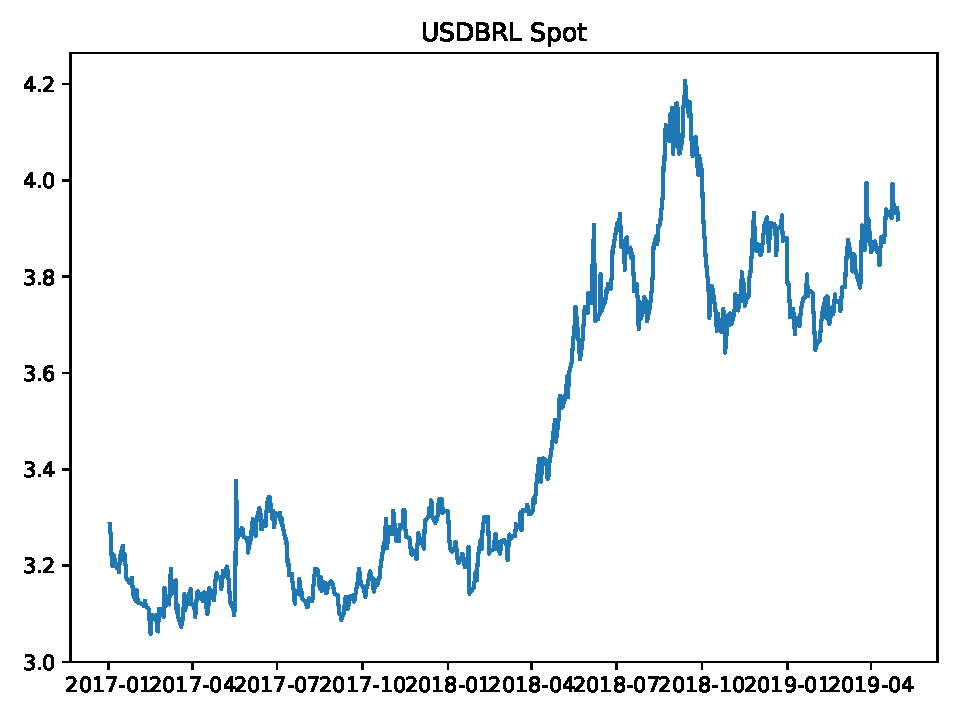
\includegraphics[width=.5\textwidth]{./figures/ECO491_HW6_Q1_Model_1.pdf}
\caption{USD/BRL spot exchange rate.}
\end{figure}

\begin{figure}[H]
\centering
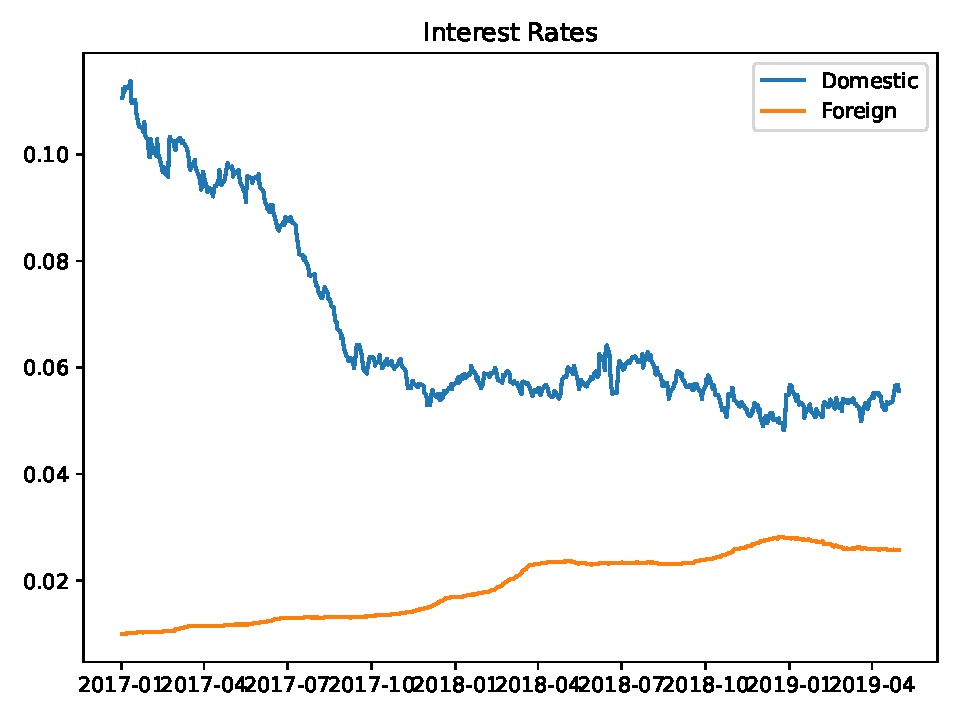
\includegraphics[width=.5\textwidth]{./figures/ECO491_HW6_Q1_Model_2.pdf}
\caption{Domestic and foreign interest rates.}
\end{figure}

\begin{figure}[H]
\centering
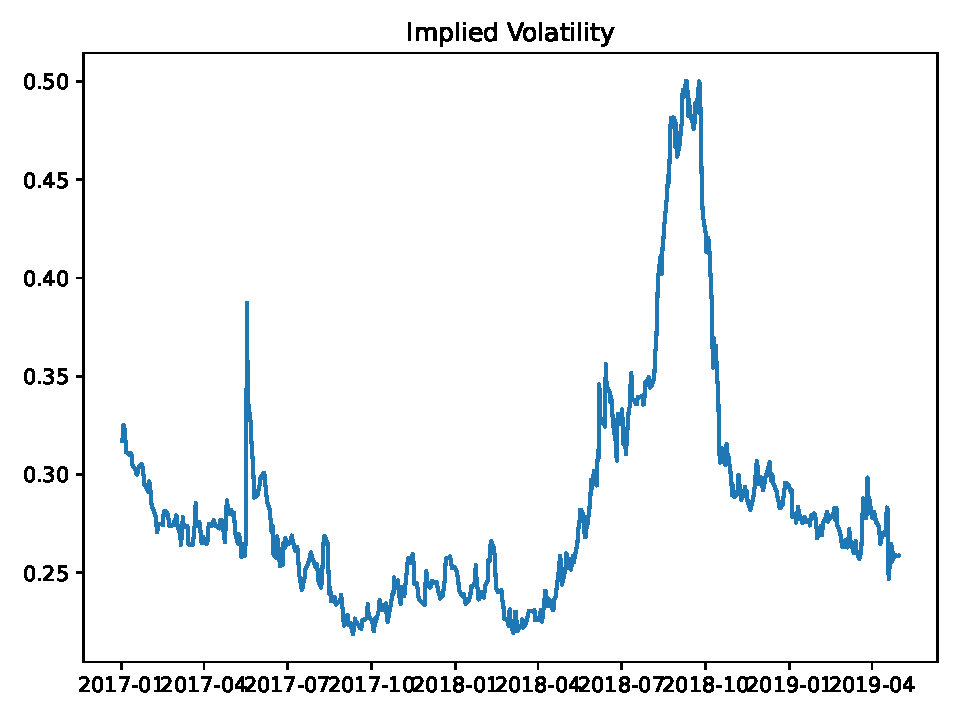
\includegraphics[width=.5\textwidth]{./figures/ECO491_HW6_Q1_Model_3.pdf}
\caption{Implied volatility.}
\end{figure}

\subsection*{1.2 \quad HS Value at Risk}

Using the full available historical dataset as a single estimation window, the
option is re-priced under each historical scenario, yielding an empirical
distribution of P\&L. The $1\%$ Historical Simulation Value at Risk is defined as
the negative $1\%$ quantile of this distribution:
\[
\mathrm{VaR}_{1\%} = - q_{0.01}(\mathrm{P\&L}).
\]

Figure~4 shows the resulting HS P\&L distribution. This measure captures the
option’s nonlinear exposure to the exchange rate, interest rates, and volatility,
as well as their empirical dependence structure.

\begin{figure}[H]
\centering
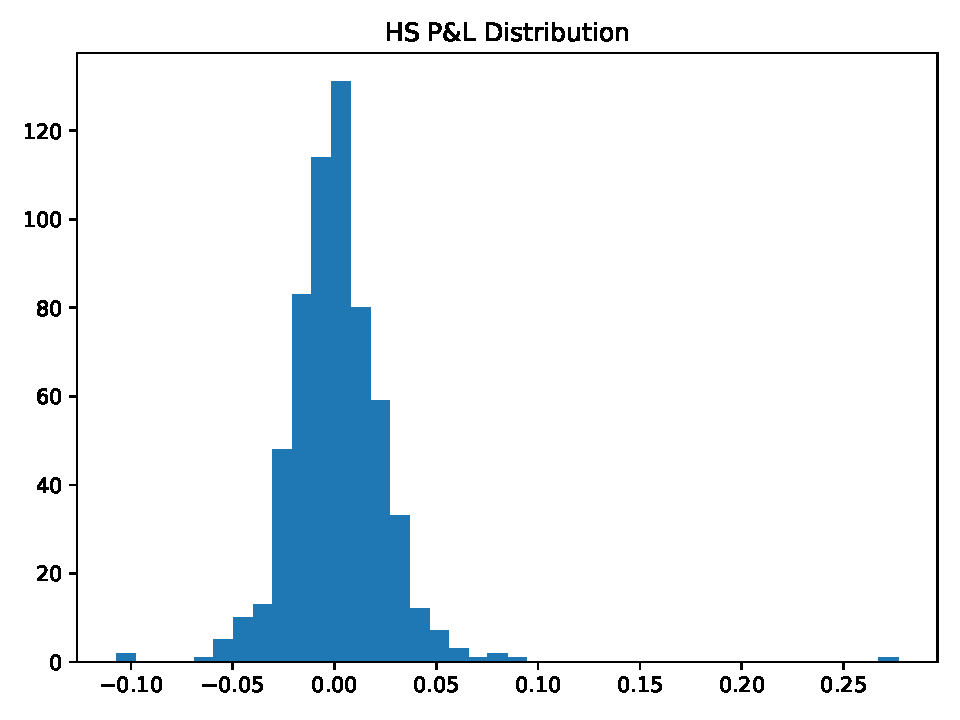
\includegraphics[width=.5\textwidth]{./figures/ECO491_HW6_Q1_Model_4.pdf}
\caption{Full-valuation HS P\&L distribution for the currency option.}
\end{figure}

% ============================================================
\section{Backtesting Value at Risk}

\subsection*{2.1 \quad HS and RiskMetrics VaR: graphical analysis}

We backtest two Value at Risk models for Apple daily log returns over the period
2015--2021: a 250-day Historical Simulation (HS) model and a RiskMetrics EWMA
model with decay parameter $\lambda=0.94$. Both models target a $1\%$ tail
probability.

At each date $t$, the VaR forecast is constructed using the previous 250 returns
and compared to the realized return $R_t$. A violation (or hit) occurs when
\[
R_t < -\mathrm{VaR}_t .
\]

Figures~5 and~6 plot realized returns together with the HS and RiskMetrics VaR
forecasts. Violations are marked at their true realized return values, allowing
direct assessment of both the frequency and severity of tail exceedances.

\begin{figure}[H]
\centering
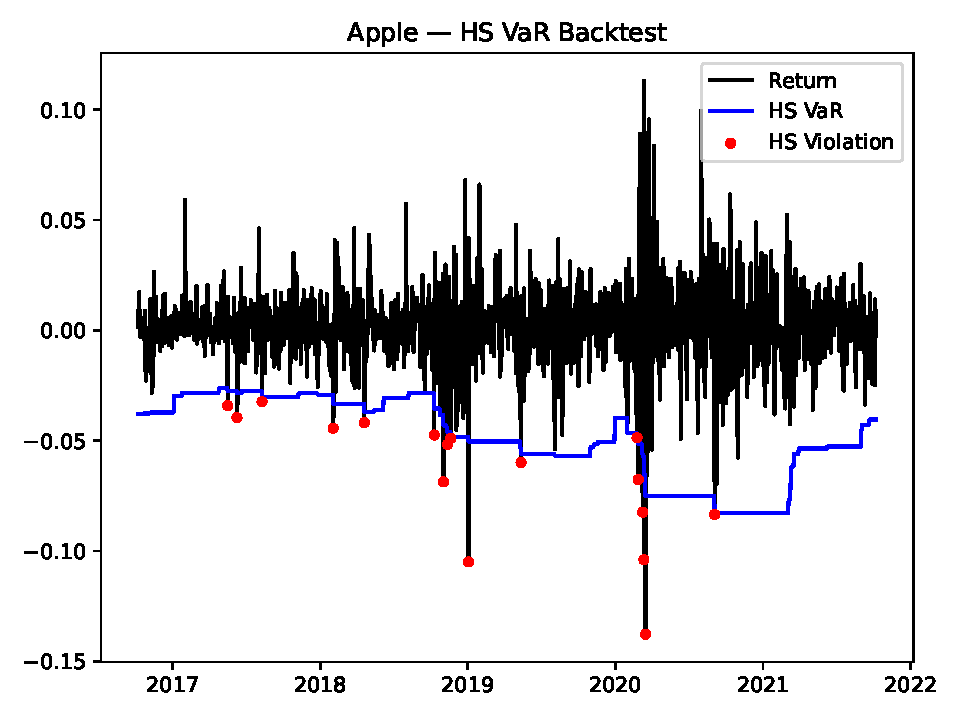
\includegraphics[width=.6\textwidth]{./figures/ECO491_HW6_Q2_Model_1.pdf}
\caption{Apple HS VaR backtest with violations overlaid.}
\end{figure}

\begin{figure}[H]
\centering
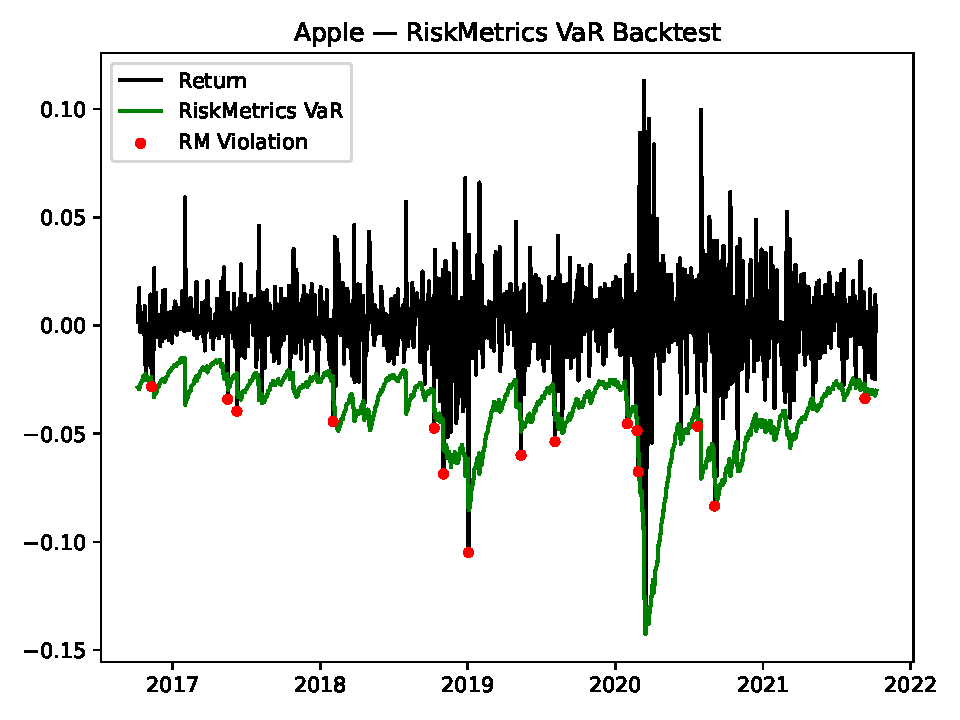
\includegraphics[width=.6\textwidth]{./figures/ECO491_HW6_Q2_Model_2.pdf}
\caption{Apple RiskMetrics VaR backtest with violations overlaid.}
\end{figure}

To further highlight the timing and magnitude of tail events, Figures~7 and~8
isolate the violations for each model. Each violation is plotted at its actual
realized return, preserving the scale of losses.

\begin{figure}[H]
\centering
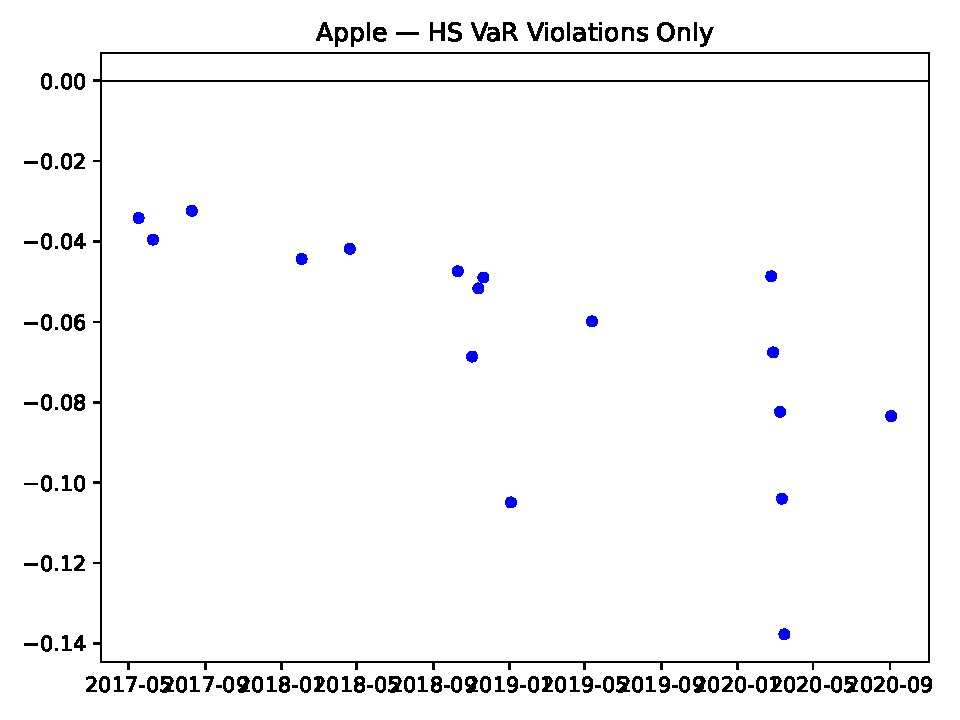
\includegraphics[width=.6\textwidth]{./figures/ECO491_HW6_Q2_Model_3.pdf}
\caption{Apple HS VaR violations only (actual returns).}
\end{figure}

\begin{figure}[H]
\centering
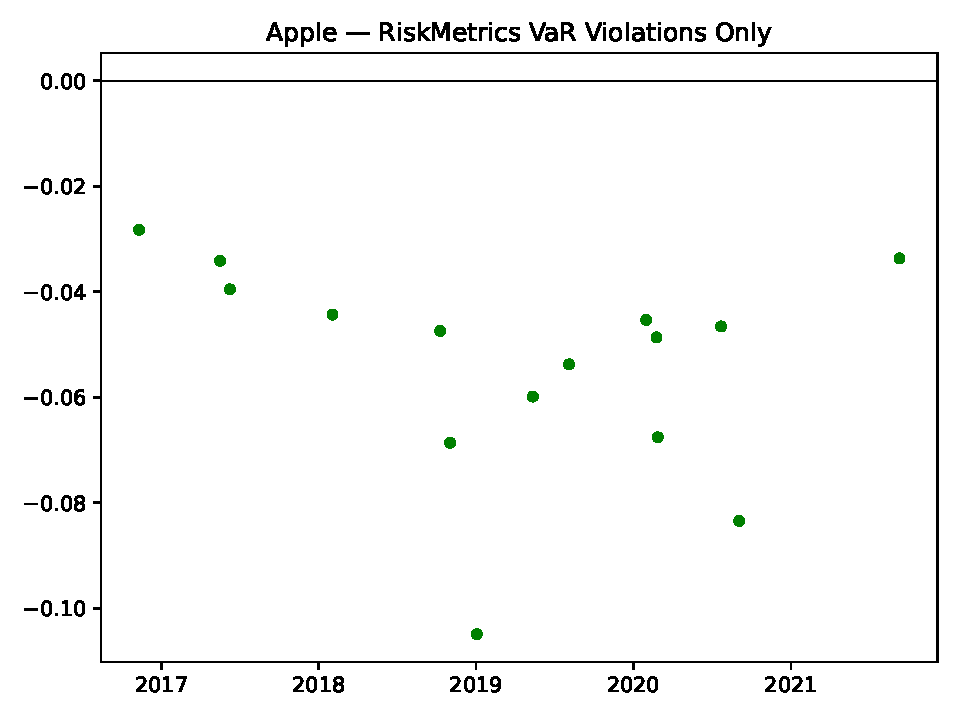
\includegraphics[width=.6\textwidth]{./figures/ECO491_HW6_Q2_Model_4.pdf}
\caption{Apple RiskMetrics VaR violations only (actual returns).}
\end{figure}

Based on these graphs, we expect approximately $1\%$ of observations to be
violations under correct calibration. If the observed violation frequency is
close to this level and violations do not exhibit excessive clustering, we would
expect the formal backtesting procedure below not to reject the model. Systematic
over- or under-frequency of violations would instead suggest rejection.

\subsection*{2.2 \quad Unconditional coverage test}

We formally assess VaR calibration using the Kupiec unconditional coverage (UC)
test. Let $I_t = \mathbf{1}\{R_t < -\mathrm{VaR}_t\}$ denote the violation
indicator. Under the null hypothesis of correct calibration, $\mathbb{P}(I_t=1)=p$
with $p=0.01$.

The UC likelihood ratio statistic is
\[
LR_{\mathrm{uc}}
=
-2 \log
\left(
\frac{(1-p)^{T-T_1} p^{T_1}}
     {(1-\hat{\pi})^{T-T_1} \hat{\pi}^{T_1}}
\right),
\quad
\hat{\pi} = \frac{T_1}{T},
\]
where $T$ is the number of backtest observations and $T_1$ is the number of
violations. Under the null, $LR_{\mathrm{uc}}$ is asymptotically $\chi^2_1$.

The test statistics computed for the HS and RiskMetrics models are compared to
the $10\%$ critical value of the $\chi^2_1$ distribution to assess whether the
observed violation frequencies are consistent with the nominal $1\%$ level.